\section{Zustandsrückführungen}

\begin{minipage}[t]{0.48\columnwidth}
    Bei einer Zustandsrückführung geht man davon aus, dass der Zustandsvektor $x$ des Systems vollständig bekannt ist und zur 
    Regelung benutzt werden kann.

    \smallskip

    \textbf{Hinweis:} Für die folgenden Betrachtungen des Systems gilt $\bm{D} = 0$, sowie

    \vspace{-0.2cm}

    $$
    \bm{K} = 
    \begin{bmatrix}
        k_1 &   k_2 & \ldots    & k_n
    \end{bmatrix}
    $$
\end{minipage}
\hfill
\begin{minipage}[t]{0.48\columnwidth}
    
    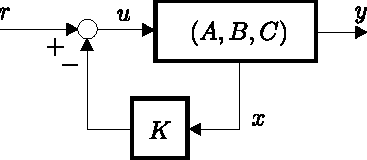
\includegraphics[width=\columnwidth, align=t]{images/ZRD_zustandsrueckfuehrung.pdf}
\end{minipage}

\medskip

\textbf{Hinweis:} Die Zeichnung zeigt das Konzept. In einem Blockdiagramm hat jede Zustandsgrösse ihre eine eigene Rückführung 
(und somit ihre eigene Verstärkung $k_i$)


Die Systemgleichung des geschlossenen Regelkreises mit \textbf{neuer Systemmatrix} $\overline{\bm{A}}$ ergibt sich zu:
$$ \dot{x} = \bm{A} \cdot x + \bm{B} \cdot u = \bm{A} \cdot x + \bm{B} \cdot \underbrace{(r - \bm{K} x)}_{u} = \underbrace{(\bm{A} - \bm{BK})}_{\overline{\bm{A}}} \cdot x + \bm{B} \cdot r $$

\medskip

Die UTF des geschlossenen Regelkreises $G_f(s)$ berechnet sich dann als:

\vspace{-0.2cm}

$$ G_f(s) = \frac{Y(s)}{R(s)} = \bm{C} \cdot (s \bm{I} - \bm{A} + \bm{BK})^{-1} \cdot \bm{B} = \bm{C} \cdot (s \bm{I} - \overline{\bm{A}})^{-1} \cdot \bm{B} $$

Wenn vorausgesetzt wird, dass das System $(\bm{A}, \, \bm{B})$ \textbf{steuerbar} ist, können die \textbf{Pole des geschlossenen Regelkreises beliebig vorgegeben} werden. \\
Dies kann mittels Polvorgabe (\ref{Polvorgabe}) oder LQR-Verfahren (\ref{LQR-Verfahren}) erreicht werden.
%-----------------------------------------------------------------------------------------------------------------------------------
\para{Geschlossener Kreis}

Für

\[
u=-Kx
\]

ergibt sich

\[
\dot x=(A-BK)x
\]

Die Eigenwerte von

\[
A-BK
\]

sind die Pole des geschlossenen Regelkreises.

\para{Polvorgabe}

Polplatzierung mittels Zustandsrückführung ist nur möglich, wenn

\[
\mathrm{rang}(Q_s)=n
\]

gilt.

\subsubsection{LQR-Regler}

Kostenfunktion:

\[
J=
\int_0^\infty
(x^TQx+u^TRu)\,dt
\]

Gewichte:

\[
Q \rightarrow Zustände
\]

\[
R \rightarrow Stellaufwand
\]

Regler:

\[
u=-Kx
\]

MATLAB:

\[
\texttt{k=lqr(A,B,Q,R)}
\]

\para{Vorverstärkung}

\[
u=-Kx+Lr
\]

\[
A_{cl}=A-BK
\]

Die Pole des geschlossenen Kreises sind die Eigenwerte von

\[
A-BK
\]
%-----------------------------------------------------------------------------------------------------------------------------------
\subsection{Eigenschaften von Zustandsrückführungen}

Reglenentwurf mittels Polvorgabe und LQR-Verfahren haben folgende Eigenschaften:

\smallskip

\begin{outline}
    \1 Zustandsrückführung wirkt sich nur auf \textbf{Pole} aus, nicht auf Nullstellen
        \2 Nullstellen, welche durch $b$-Koeffizienten bestimmt sind, belieben erhalten
    \1 Ordnung des Regelkreises bleibt erhalten ( \textrightarrow\ statischer Regler)
    \1 Zustandsrückführung $k$ entspricht grundsätzlichen einem statischen (P-)Regler.
        \2 Bei konstanter Führungsgrösse $r$ entsteht ein stationärer Fehler \\
            \textrightarrow\ kann durch Erweiterung mit Vorverstärkung oder I-Anteil in Regelkreis korrigiert werden (siehe Abschnitt \ref{Statische Erweiterungen der Zustandsrückführung})
\end{outline}


\subsection{Reglerentwurf mittels Polvorgabe}{194-196}
\label{Polvorgabe}

Bei der Zustandsrückführung können \textbf{alle $\bm{n}$ Pole beliebig vorgegeben} werden, sofern das \textbf{System steuerbar} ist.

\smallskip

Bei einer WOK hingegen hat man meist nur einen Freiheitsgrad (Verstärkungsfaktor des Reglers), um alle $n$ Pole festzulegen, 
da die Pollagen miteinander gekoppelt sind.


\subsubsection{Lage der Pole}

\begin{minipage}[t]{0.35\columnwidth}
    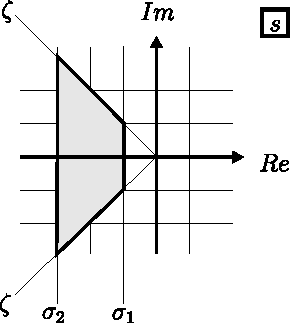
\includegraphics[width=\columnwidth, align=t]{images/ZRD_polplatzierung.pdf}
\end{minipage}
\hfill
\begin{minipage}[t]{0.62\columnwidth}
    \raggedright
    Die Wahl der Pole des Reglers soll folgende Kriterien erfüllen:

    \smallskip

    \begin{outline}
        \1 Pole müssen in LHE liegen $(\sigma < 0)$, damit Regelkreis stabil ist
        \1 Transienten sollen schneller abklingen als ein geeignetes $C \cdot e^{- \sigma_1}$
        \1 System soll genügend gedämpft sein, z.B. $\zeta > \frac{1}{\sqrt{2}}$
        \1 Obere Grenze $\sigma_2 > \sigma$ verhindert zu grosse Stellsignale
        \1 Pole, welche bereits akzeptabel liegen nicht unnötig verschieben
    \end{outline}
\end{minipage}


\subsubsection{Vorgabe der Pollagen}

Die Eigenwerte der Matrix $\overline{\bm{A}} = (\bm{A} - \bm{BK})$ sind gegeben durch die \textbf{Wurzeln} (Nullstellen) des Polynoms

\vspace{-0.2cm}

$$ \boxed{ \det \left(\lambda \cdot \bm{I} - \overline{\bm{A}} \right) = \det \left( \lambda \cdot \bm{I} - \bm{A} + \bm{BK} \right) = (\lambda - \lambda_1) \cdot  (\lambda - \lambda_2) \ldots  (\lambda - \lambda_n) } $$

Das geregelte System bzw. der geschlossene Regelkreis besitzt die UTF $G_f(s)$, bei welcher der \cbl{Nenner} bzw. die Pole vorgegeben werden.
$$ G_f(s)   = \frac{Y(s)}{U(s)} 
            = \frac{b_{n-1} s^{n-1} + b_{n-2} s^{n-2} + \ldots + b_1 s + b_0}{\cbl{ s^n + (a_{n-1} + k_n) s^{n-1} + \ldots + (a_1 + k_2) s + (a_0 + k_1) } } $$ 

Um die Pole des geregelten Systems $G_f(s)$ an die vorgegeben Stellen $\lambda_1 \ldots \lambda_n$ zu bringen, müssen folgende Polynome
mittels \textbf{Koeffizientenvergleich} zum Übereinstimmen gebracht werden. (Das Polynom rechts wird sinnvollerweise ausmultipliziert.)

\vspace{-0.2cm}

$$ \boxed{ \cbl{ s^n + (a_{n-1} + k_n) s^{n-1} + \ldots + (a_1 + k_2) s + (a_0 + k_1)} \overset{!}{=}
\det \left( s \cdot \bm{I} - \bm{A} + \bm{BK} \right) } $$

\textbf{Hinweis:} Die Parameter $k_i$ sind \textbf{eindeutig} bestimmbar, sofern das System \textbf{steuerbar} ist.


\example{Struktur eines Regelkreises mit Zustandsrückführung}

\begin{center}
    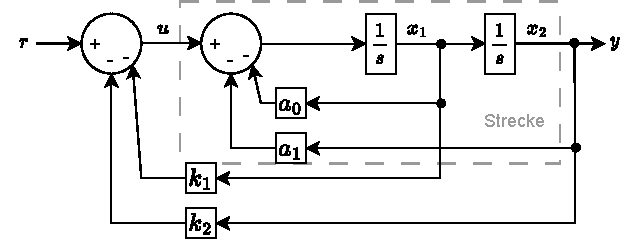
\includegraphics[width=0.7\columnwidth]{images/ZRD_zustandsrueckfuehrung_beispiel.pdf}
\end{center}

\vspace{-0.2cm}


\subsection{LQR-Verfahren (Linear Quadratic Regulator)}{196-199}
\label{LQR-Verfahren}

Für die Zustandsrückführungen wird die Matrix $\bm{K}$ mit Einträgen $k_i$ benutzt. Nun kann es sein, dass mehrere Matritzen $\bm{K}$ zur gleichen
Polverteilung führen. \\
\textrightarrow\ Das (Linear Quadratic Regulator) LQR-Verfahren ermittelt die \textbf{beste Matrix} $\bm{K}$

\medskip

Das LQR-Verfahren beruht auf der Lösung eines \textbf{Optimierungsproblems}. 
Aus folgenden beiden Anforderungen muss ein 'optimaler' Kompromiss gefunden werden:

\smallskip

\begin{outline}
    \1 Zustände $x(t)$ sollten möglichst schnell gegen $0$ konvergieren
    \1 Stellgrösse $u(t)$ soll nicht zu gross werden (nicht zu viel Stellenergie brauchen)
\end{outline}


\subsubsection{Zielfunktion $\bm{J(K)}$}

Die Zielfunktion $J(K)$ soll \textbf{minimiert} werden, um optimale Gewichtungsfaktoren $k_i$ für die Zustandsrückführungen zu finden. \\
Dabei setzt sich die Zielfunktion $J(K)$ aus den Zuständen $(x_1, \, \cdots, \, x_n)$ und den Eingangssignalen $(u_1, \, \cdots, \, u_m)$, 
sowie Gewichtungsmatritzen $\bm{Q}$ und $\bm{R}$ zusammen.

\begin{minipage}[c]{0.69\columnwidth}
    $$ \boxed{J(K) = \int\limits_{0}^{\infty} \left[ x(\bm{K}, t)^T \cdot\bm{Q} \cdot x(\bm{K}, t) + u(\bm{K}, t)^T \cdot \bm{R} \cdot u(\bm{K}, t) \right] \, \diff t } $$
\end{minipage}
\hfill
\begin{minipage}[c]{0.3\columnwidth}
    \begin{outline}
        \1 $\bm{Q}$ gewichtet Zustände \\
            Dimension: $n \times n$
            \smallskip
        \1 $\bm{R}$ gewichtet Eingänge \\
            Dimension: $m \times m$
    \end{outline}
\end{minipage}



\subsubsection{Wahl der Gewichtungsmatritzen $\bm{Q}$ und $\bm{R}$}

Die Matritzen $\bm{Q}$ und $\bm{R}$ werden folgendermassen gewählt:

\smallskip

\begin{outline}
    \1 Falls möglich: Diagonalmatritzen
        \2 Elemente auf \textbf{Diagonalen} müssen \textbf{positiv} sein \textrightarrow\ positiv definit
    \1 Falls keine Diagonalmatrix: Symmetrie
\end{outline}

\smallskip

\textbf{Hiweis:} In der Praxis ist die Wahl von $\bm{Q}$ und $\bm{R}$ meist ein \textbf{iterativer Prozess}. \\
Der 'erste Wurf' der Werte in den Matritzen wird so gewählt, dass \textbf{alle Summanden des Integranden in etwa gleich gewichtet} sind.


\example{Zielfunktion mit zwei Zuständen und einem Eingang}

Die Grössen liegen in den vorgegebene Bereichen.
Mit den Gewichtungsmatritzen sollen die Anteile der drei Integranden in vergleichbare Grösenordnungen gebracht werden.

\begin{ctabular}{l l l}
    \tabitem $x_1(t) \approx \pm 5 \cdot 10^{-3} \, \meter$         &
    \tabitem $x_2(t) \approx \pm 10^{2} \, \frac{\meter}{\second}$  &
    \tabitem $u(t) \approx \pm 10 \, \volt$
\end{ctabular}

\vspace{-0.3cm}

$$ \text{Integranden auf Gewichtung 1 bringen:} \quad \cbl{200^2} \cdot x_1^2 + \cor{100^2} \cdot x_2^2 + \cgn{0.1^2} \cdot u^2 $$

\vspace{-0.3cm}

\[
    \text{In Matrixform:} \quad 
    J = \int\limits_{0}^{\infty} \left[ x^T \cdot
    \begin{bmatrix}
        \cbl{4 \cdot 10^4}  & 0         \\
        0                   & \cor{10^4} 
    \end{bmatrix}
    \cdot x + u^T \cdot
    \begin{bmatrix}
        \cgn{10^{-2}}
    \end{bmatrix}
    \cdot u \right] \, \diff t
\]


\example{Nicht-Diagonale Matrix $\bm{Q}$}

Mischterme stehen neben der Diagonalen und werden aufgeteilt.

\vspace{-0.2cm}
\[
    \cbl{13} \cdot x_1^2 + \cvt{(-16)} \cdot x_1 \cdot x_2 + \cor{15} \cdot x_2^2
    \qquad 
    \Rightarrow\
    \begin{bmatrix}
        x_1 & x_2
    \end{bmatrix}
    \cdot
    \begin{bmatrix}
        \cbl{13}    & \cvt{-8}  \\
        \cvt{-8}    & \cor{15}
    \end{bmatrix}
    \cdot
    \begin{bmatrix}
        x_1 \\ x_2
    \end{bmatrix}
\]


\subsubsection{Optimale Rückführverstärkungen $\bm{K}$}

Der geschlossene Regelkreis mit Zustandsrückführung (also mit \textbf{neuer Systemmatrix} $\overline{\bm{A}}$) gehorcht der Differentialgleichung 

\vspace{-0.2cm}

$$ \dot{x} = \bm{A} \cdot x - \bm{BK} \cdot x = (\bm{A} - \bm{BK}) \cdot x \qquad \text{mit } x(0) = x_0 $$


und hat die Lösung

\vspace{-0.2cm}

$$ x(\bm{K}, t) = e^{(\bm{A} - \bm{BK}) t} \cdot x_0 \qquad \qquad
    u(\bm{K}, t) = - \bm{K} \cdot x(\bm{K}, t) = - \bm{K} \cdot e^{(\bm{A} - \bm{BK}) t} \cdot x_0 $$


\vspace{0.2cm}

Damit wird die Zielfunktion $\bm{J(K)}$ 

\vspace{-0.4cm}

\begin{align*}
    J(K)    &= \int\limits_{0}^{\infty} \left[ x(\bm{K}, t)^T \cdot\bm{Q} \cdot x(\bm{K}, t) + u(\bm{K}, t)^T \cdot R \cdot u(\bm{K}, t) \right] \, \diff t \\
            &= x_0^T \cdot \underbrace{ \int\limits_{0}^{\infty} \left[ e^{(\bm{A} - \bm{BK}) t} \right]^T \cdot \left[ \bm{Q} + \bm{K^T RK} \right] \cdot e^{(\bm{A} - \bm{BK}) t} \, \diff t }_{\bm{S}(\bm{K})} \cdot x_0
\end{align*}


Die optimalen Rückführverstärkungen (als Matrix $\bm{K}$) ergeben sich aus der positiv definiten Lösung der Matrix $\bm{S}$ der entsprechenden Matrix-Ricatti-Gleichung:

\vspace{-0.2cm}

$$ \boxed{ \bm{K} = \bm{R^{-1} B^T S} } $$

\textbf{Hinweis:} Meist wird die Lösung $\bm{K}$ direkt mit Matlab ermittelt.


\subsubsection{Eigenschaften des LQR-Verfahrens}

\begin{outline}
    \1 Ist $\bm{R}$ \textbf{'klein'}, ergibt sich tendentiell eine \textbf{grössere Reglerverstärkung $\bm{K}$} und ein schnellerer Regelkreis
        \2 Pole liegen weiter links
    \1 Werden $\bm{Q}$ und $\bm{R}$ um denselben Faktor geändert, so ergibt sich wieder dieselbe Rückführungsverstärkung $\bm{K}$
    \1 Gelegentlich ist es von Vorteil, als Gewichtung $\bm{Q} = \bm{C^T C}$ zu verwenden
        \2 $\bm{C}$ entspricht der 'richtigen' Ausgangsmatrix des Systems
    \1 Mittels LQR-Verfahren werden sehr \textbf{robuste Regler} entworfen (\textrightarrow\ siehe Skrip S. 199)
\end{outline}


\medskip

\paragraph{Einfluss von $\bm{R}$ und $\bm{Q}$ auf Stellgrösse $\bm{u(t)}$}

\begin{ctabular}{l c c}
    \toprule
    $\bm{R} \uparrow$ / $\bm{Q} \downarrow$ & $u(t=0) \, \downarrow$    & langsameres Abklinken \\
    \midrule
    $\bm{R} \downarrow$ / $\bm{Q} \uparrow$ & $u(t=0) \, \uparrow$      & schnelleres Abklinken \\
    \bottomrule
\end{ctabular}

%-----------------------------------------------------------------------------------------------------------------------------------
\subsubsection{Zustandsregler mit PI-Zusatz}

Integratorzustand:

\[
x_I=\int e(t)\,dt
\]

Erweiterter Zustandsvektor:

\[
x_{PI}
=
\begin{bmatrix}
x\\
x_I
\end{bmatrix}
\]

Regler:

\[
u=-Kx-k_Ix_I
\]

Vorteil:

\[
e_\infty = 0
\]

für konstante Führungs- und Störgrössen.
%-----------------------------------------------------------------------------------------------------------------------------------

\subsection{Statische Erweiterungen der Zustandsrückführung}
\label{Statische Erweiterungen der Zustandsrückführung}

Die Zustandsrückführung sorgt dafür, dass der geschlossene Regelkreis $G_f(s)$ eine befriedigende Dynamik hat.
Das (statische) \textbf{Folgeverhalten} ist jedoch noch \textbf{nicht garantiert}. \\
Für den geschlossenen Regelkreis $G_f(s)$ soll gelten:

\smallskip

\begin{outline}
    \1 Führungsverhalten: $y = r$
    \1 Keine Regelabweichung bei konstantem $r$: $e(t) = r(t) - y(t) \to 0$ bzw. $G_f(0) = 1$ 
\end{outline}

\smallskip

\textbf{Hinweis:} Folgende Betrachtungen beziehen sich auf SISO-Systeme.


\subsubsection{Erweiterung mit Vorverstärkung}{200}

$L$ kann verwendet werden, um $r = y$ zu garantieren. \\
Ausserdem kann $L$ als Vorfilter verwendet werden, und so die Dynamik des Regelkreises verbessern 
\textrightarrow\ Lead-Glied mit $T_2 < T_1$ macht Regelkreis schnell

\smallskip

\begin{minipage}[t]{0.63\columnwidth}
    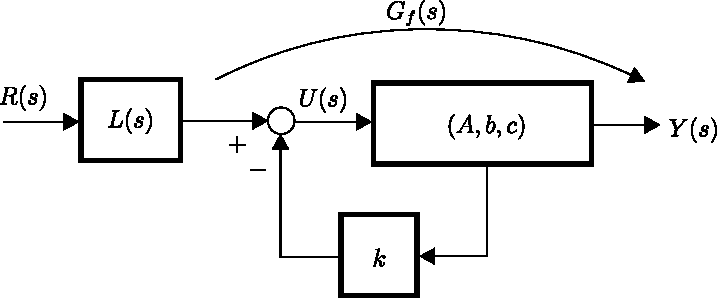
\includegraphics[width=\columnwidth, align=t]{images/zustandsrueckfuehrung_vorverstaerkung.pdf}
\end{minipage}
\hfill
\begin{minipage}[t]{0.33\columnwidth}
    \textbf{Verstärkung korrigieren:}
    $$ L = G_f(0)^{-1} = \frac{1}{G_f(0)} $$

    \textbf{Zusätzliches Vorfilter:}
    $$ L = \frac{1}{G_f(0)} \cdot \frac{s T_1 + 1}{s T_2 + 2} $$
\end{minipage}

\medskip

$$ \text{UTF Regelkreis (ohne  L(s)):} \quad G_f(s) = \frac{Y(s)}{U(s)} = \bm{C} \cdot (s \bm{I} - \bm{A} + \bm{BK})^{-1} \cdot \bm{B} = \bm{C} \cdot (s \bm{I} - \overline{\bm{A}})^{-1} \cdot \bm{B}$$

Die Vorverstärkung hat jedoch den \textbf{Nachteil der Parameterabhängigkeit}.


\subsubsection{Erweiterung mit PI- / I-Zusatz}{200-202}

Der statische Fehler kann auch mittels PI- bzw. reinem I-Anteil im Regler ($K_P = 0$) unterdrückt werden.
Der Entwurf eines solchen zusätzlichen Reglers kann auf zwei verschiedene Arten erfolgen.

\smallskip

Die Integratorerweiterung hat jedoch den \textbf{Nachteil der Phasensenkung}.

\medskip

\paragraph{Variante: Kaskadierter Regler}

Der Entwurf des Reglers erfolgt in zwei \textbf{separaten} Schritten:

\smallskip

\begin{enumerate}
    \item Zustandsrückführung $\bm{K}$ entwerfen
    \item PI-Regler für den in Schritt 1 entstandenen Regelkreis entwerfen
\end{enumerate}

\smallskip

\textrightarrow\ \textbf{Nicht ideal}, da z.B. die robusten Eigenschaften des inneren Kreises in Schritt 2) verloren gehen können

\vspace{-0.2cm}

\begin{center}
    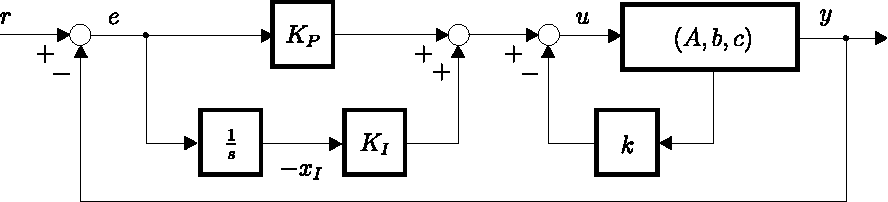
\includegraphics[width=0.8\columnwidth]{images/zustandsrueckfuehrung_PI.pdf}
\end{center}


\paragraph{Variante: Erweiterung der Strecke}

Eine bessere Variante ist es, den Regler 'aus einem Guss' zu entwerfen, indem die \textbf{Stecke} $n$-ter Orndung (aus obiger Abbildung)
\textbf{um einen Integrator erweitert} wird.

\smallskip

Der Zustandsvektor der neuen Strecke wird wegen dem zusätzlichen Integrator um den Zustand $x_I$ erweitert. Das System hat folgende ZRD:

\vspace{-0.1cm}

$$
\underbrace{ \begin{bmatrix} \dot{x} \\ \dot{x}_I \end{bmatrix}}_{\dot{x}_{\rm PI}}
=
\underbrace{\begin{bmatrix} \bm{A} & 0 \\ c & 0 \end{bmatrix} }_{\bm{A}_{\rm PI}}
\cdot
\underbrace{ \begin{bmatrix} x \\ x_I \end{bmatrix} }_{x_{\rm PI}}
+
\underbrace{ \begin{bmatrix} b \\ 0 \end{bmatrix} }_{b_{\rm PI}} \cdot u
\qquad \qquad 
y
=
\underbrace{ \begin{bmatrix} c & 0 \end{bmatrix}}_{c_{\rm PI}} \cdot x_{\rm PI}
$$


Für die neue Strecke kann anschliessend eine Zustandsrückführungsmatrix $\bm{K}$ ausgelegt werden. 
Dafür können Polplatzierung oder das LQR-Verfahren angewendet werden.

\vspace{-0.1cm}

$$ u = -(k + K_P \cdot c) \cdot c - K_I \cdot x_I = - \underbrace{ \begin{bmatrix} k + K_P \cdot c & K_I \end{bmatrix}}_{k_{\rm PI}} \cdot \underbrace{ \begin{bmatrix} x \\ x_I \end{bmatrix} }_{x_{\rm PI}} $$


\begin{outline}
    \1 Regler-Parameter $K_I$ entspricht letztem Element des Vektors $k_{\rm PI}$
    \1 Sobald der freie Parameter $K_P$ festgelegt ist, ist der Vektor $k_{\rm PI}$ eindeutig definiert
\end{outline}

\smallskip

Sobald die Werte $K_P$ und $K_I$ festgelegt sind, wird der Regler gemäss obiger \textbf{Kaskaden-Struktur} implementiert

